How should a developer choose a package from among many choices?
This question gets more difficult each day as new open source packages are published.
We want to build visualizations and search tools to help developers make such choices more quickly and effectively.

We start by asking what information matters to developers.
Typically, developers choose open source packages based on functionality and quality of documentation.
We suggest that as social communication channels become intertwined with the development process~\cite{storey_revolution_2014},
developers need to understand the ``social health'' of a package's community before they use it.
We define a package as \textit{socially healthy} when a developer can reliably get helpful answers from a package's forums, mailing lists, and other communication channels.

We ran a study to find out how developers currently learn about the social health of packages.
We contribute preliminary results from this study, including the following:
(1) Developers seek out common cues when answering the same questions about a package's social health;
(2) They rely on texts of issue reports, documents, and conversations to assess social health.

\begin{figure*}
\centering
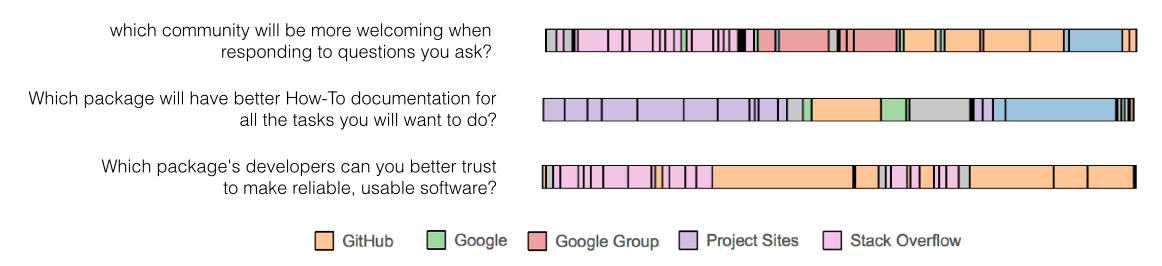
\includegraphics[width=0.98\textwidth]{figures/visits}
\caption{%
We asked developers to answer questions about the social health of open source projects,
specifically their community, documentation, and developers.
This plot shows the search behavior of a single participant for three of the six questions.
This participant viewed many documents to judge the difference in social health between two packages.
To determine which package had a more welcoming community, they viewed seven questions on Stack Overflow, four issues on GitHub, and three conversations on Google Groups.
}
\label{fig:visits}
\end{figure*}
